\documentclass[a4paper,10pt,titlepage,twocolumn]{article}
    \usepackage[left=1in,right=1in,top=1in,bottom=1in]{geometry}
    \usepackage{graphicx}
    \usepackage{url}
\begin{document}
\linespread{1.5}
    \title{COMP90015 Distributed Systems \\Project 1 Bitbox\\}
    \author{\\\Large \textit{Team Koala} \\
    \\
        \begin{tabular}{|c|c|c|}
        \hline
        Members &loginName&Emails \\ \hline
        Yue Guo & guoy7 &\url{guoy7@student.unimelb.edu.au}  \\ 
        Runze Nie & runzen & \url{runzen@student.unimelb.edu.au} \\
        Cheng Qian & cqq & \url{cqq@student.unimelb.edu.au} \\ \hline
    \end{tabular}}
    \date{}
    \maketitle
    
    \section*{Introduction}
    This project is about a system named ‘bitbox’ which syncs files between peers in an unstructured P2P Network. The system communicates with peers via persistent TCP connections and monitors directories and files to process to events including file create, delete and modify. Contents are transferred inside JSON using Base64 encoding with asynchronous request/reply between peers.
    \\Firstly, the contents of files need to be transferred as bytes with encoding and decoding via Base64. This is going to strengthen the security of this system. Additionally, the system needs to use a Breadth-first search to find peers and create asynchronous requests/replies between peers.
    \\Through working on this project, some general technical skills like managing codes with Git and managing the project with maven are trained. Moreover, the project enhanced the understanding of the principles in distributed systems.
    

    
    \section*{Fault detection/Tolerance/ Recovery}
    Firstly, the connection may not be established at first which means peers are not structured as a P2P network. Moreover, the system can be impacted by receiving invalid protocols. This kind of protocols can be wrong or appear in the wrong place. Additionally, the connection may fail due to many uncontrollable factors. For example, connections between peers may be forced terminated while one of the peers shutdowns or offline from the internet. When this happened, the files which had not completed transmission will exist as temporary files. These files will be detected as files which are already existing and not continue transferring.
    \\The system will timeout from the connection which is not established and going to listen on other peers on the designed port. This helps the system going back to the right way and running continuously. When the systems meet invalid protocols, it is designed to throw exceptions and print to logs for these situations so that webmaster can notice and troubleshoot problems. Almost all kinds of invalid protocols are considered when designing this system so this fault can be tolerated and will not impact the system much. It will be more severe when the connection is interrupted during transmission. The system is not able to handle this fault now. Users may need to delete these files manually. 
    \\However, this fault can be handled with breakpoint resume function in the future. The system can hold the data of how many chunks have been transferred and resume the transmission, which likes how BitTorrent works. Plus, temporary files should be detected and deleted when it does not exist in any peer. Both of these revisions will help the system to recover from the fault caused by interrupting transmission.

    \section*{Scalability}
    According to the given design of the protocol, the increase in the number of peers might lead to certain problems and have significant impacts on the performance of the system.
    \\The first one is concerned with the maximum number of incoming connections. As each peer in the BitBox system has a limit on the maximum number (max) of incoming connections, when there are n ($n \geq max$) peers connecting to each other, the newcomers will always only have the max latest connected peers to connect to. Therefore, the distance between the peer coming first and the one coming last would be continuously increasing, with the growing of peers’ number, which means the changes of the files occurring in the first peer might take an unacceptably long time to be synchronized in the last peer, and hence the performance of the system is lost.
    \\To deviate the impact of this issue, a number of peers could be set as “core peers”, which have a much larger maximum number of incoming connections than the normal ones, and the newcomers will try to reach these “core peers” first, then the others. Thus, the distance between any two peers has the possibility to be reduced (Figure \ref{fig:1}).
    \begin{figure}[htbp] 
        \centering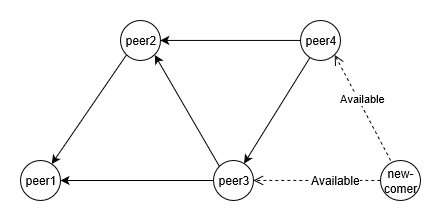
\includegraphics[width=2.5in]{picture.jpg} 
        \caption{Net of Connections between Peers $(max = 2)$}\label{fig:1} 
    \end{figure} 
    \\Another issue of the BitBox system is concerned with message transmission and process. As the peers in the BitBox system are performing as both the server and the client, they must receive and send multiple messages simultaneously, through multiple connections to the other peers. Therefore, when the connections increase, the speed of message transmission would be limited by the bandwidth the peer has. Moreover, because each connection is allocated to a thread in this system, considerable numbers of threads within a peer might reduce the processability of each individual thread. The result would be the delay of the information transmitted, and hence the concurrency might not be ensured.
    \\To handle this problem, other than limiting the maximum number of incoming connections for each peer, the protocol might also need to reduce the overhead, for instance, certain responses such as $DIRECTORY\_DELETE\_RESPONSE$ and $DIRECTORY\_CREATE\_RESPONSE$ may need not to be sent if the operation succeeds and the 'status' is true.

    \section*{Security}
    In this P2P system, The first security issue is information disclosure. At the synchronization phase, the connected two peers might have the files with the same pathname but different content. In this case, it is tricky to decide which file should be kept and which file should be abandoned, or else, whether both files should be kept or eliminated, or even mixed. Each of these divisions is possible to bring the issue referred to as information leakage. 
    \\Moreover, since peers do not need to be authorized and all the resources are shared, information disclosure becomes a serious security issue. During the reading file phase, when a peer receives a $FILE\_BYTES\_REQUEST$, it contains the IP address of the sender, which is not authorized. Then that peer reads the content from the specific file and sends the content to the sender. In this case, the information is easy to be disclosed. Furthermore, during the writing file phase, a peer might receive some aggressive information or the trojan virus. 
    \\Another serious security issue is the messages intercepted by unauthorized peer. This issue would lead to IP address leakage, message tampering, resend these messages to attack protocol loophole or denial of service attack. For instance, an unauthorized peer tampers a common document, which could cause information loss, or when a peer is transferring a large file to another peer, if the unauthorized peer changes or deletes that file, there will be misread of the file.
    \\As for information leakage, it seems to be unavoidable in any network. However, in the first situation mentioned above, it can be fixed by implementing the file system manager and protocol properly. Our group decided to save the file that has a larger ’lastModified’, i.e. the latest modified one, which can be easily achieved by using ‘modifyFileLoader’ and $FILE\_CREATE\_REQUEST$ protocol. Moreover, cryptography the protocol might decrease the possibility of information leakage.
    \\However, in terms of authorizing and intercepting messages, the current system is not able to reach an acceptable situation easily. To improve the system in terms of this aspect, the peer sending the connection request needs to be authorized by the receiver, and every file or directory request needs to be agreed by the request receiver.


    \section*{Challenges}
    In spite of the issues described above, the transparency is another important challenge related in this system. With transparency, a distributed system conceals its separation of components from users and application programmers, which means it could perform like a local system.
    \\One essential type of transparency relevant in the BitBox system is the access transparency, which requires the remote resources can be accessed as if they are the local ones. In this project, although the resources for each peer are stored locally, the operation on these files, such as creation, deletion, and modification, can be detected and spread to other peers for synchronization. Thus, the remote resources are also able to be changed and perform like the local ones.
    \\The BitBox system conceals the majority of failures before, during and after the connection. For instance, the refused connection failure, which is caused by reaching the maximum number of incoming connections in the remote peer, will be caught and dealt with by doing a breadth-first search of other might available peers. Therefore, failure transparency is implemented in this system.
    \\However, there are several types of transparency which are best to have or can be improved in the BixBox system. For instance, performance transparency enables the system to be scalable, which means its performance would not be reduced as the number of users or connections increase significantly. In the BixBot system, setting the default limit for the incoming connections might be supposed to handle this issue, but this limitation is a fixed number. Therefore, to improve performance transparency, the protocol could be modified to enable this number to vary as the loads change.
    \\The location transparency is also not implied in this system, as the user should know the network location, such as   (IP addresses) and the port numbers, of the peers to connect to. To make the BitBox system capable with this transparency, the program could be embedded with default peer IP addresses for initial connections.


\end{document}